\documentclass[12pt]{paper}

\usepackage{tikz}
%\usepackage{Schwieg}
\usepackage[margin=1in]{geometry}
\usepackage{pgfplots}

\usepackage{float}
\usepackage{amsmath}
\usepackage{bm}
\usepackage{amsthm}
\usepackage{mathtools}
\usepackage{amsfonts}
\usepackage{bbm}
\usepackage{graphicx}

\DeclareMathOperator{\diam}{diam}
\DeclareMathOperator{\interior}{int}
\DeclareMathOperator{\close}{cl}

\newcommand{\met}[1]{d \left ( #1 \right )}
\newcommand{\brak}[1]{ \left [ #1 \right ] }
\newcommand{\cbrak}[1]{ \left \{ #1 \right \}}
\renewcommand{\vec}[1]{ \bm{ #1 }}
\newcommand{\abs}[1]{\left \lvert #1 \right \rvert}
\newcommand{\seq}[1]{{\left \{ #1 \right \}}}
\newcommand{\conj}[1]{ \overline{ #1 } }
%\newcommand{\close}[1]{ \bar{ #1 } }
\newcommand{\set}[1]{\left \{ #1 \right \}}
\newcommand{\Lim}{\lim\limits}
\newcommand{\compose}{\circ}
\newcommand{\inv}[1]{{#1}^{-1}}
\newcommand{\compl}[1]{{#1}^{c}}



\newcommand{\setR}{ \mathbb{R} }
\newcommand{\setQ}{ \mathbb{Q} }
\newcommand{\setZ}{ \mathbb{Z} }
\newcommand{\setN}{ \mathbb{N} }

\newcommand{\plim}{ \overset{p}{\to} }
\newcommand{\mean}[2][N]{ \overline{ #2 }_{#1}}
\newcommand{\exV}[1]{\mathbb{E} \left [ #1 \right ]}
\newcommand{\Vari}[1]{\mathbb{V} \left ( #1 \right )}

\newcommand{\est}[2][n]{ \widehat{ #2 }_{#1}}
\newcommand{\altest}[2][n]{ \tilde{ #2 }_{#1}}

\newcommand{\indicate}[1]{ \mathbbm{1}_{\{#1\}}}
\newcommand{\convDist}{ \overset{d}{\to}}
\newcommand{\unif}{\emph{U}}
\newcommand{\normal}{\mathcal{N}}
\newcommand{\eye}{\mathbbm{I}}

\newcommand{\bigO}{\mathcal{O}}
\newcommand{\Lagrange}{\mathcal{L}}

\newcommand{\deriv}[2]{\frac{ \partial #1}{ \partial #2}}

\DeclarePairedDelimiter{\ceil}{\lceil}{\rceil}
\DeclarePairedDelimiter{\floor}{\lfloor}{\rfloor}
\DeclarePairedDelimiter{\norm}{\lVert}{\rVert}


\begin{document}

\section*{Question 1}
Provide the intuition as to why the solution to (1) is the $\tau^{th}$
quantile of $Y$. Think about the shape of $\rho_{\tau}$, where the loss is
greatest and how that depends on $\tau$.
\vspace{.3in}

We can think of the check function $\rho_{\tau}$ as a function that weighs
over and under-estimation differently. The loss
is linear to both the left and right of zero. We can see a plot of the
check function for $\tau= .3$ below

\begin{figure}[H]
  \centering
      \caption{$\rho_{\tau}, \tau = .3$} 

\begin{tikzpicture}
  
  \begin{axis}[xmin=-1,xmax=1,ymin=0,ymax=1, samples=100,domain=-1:1]
    % \addplot(x,.5*(x-abs(x)/x));
    \addplot[thick](x,{x*(.3 - .5*(x-abs(x))/x)});
  \end{axis}
\end{tikzpicture}
\end{figure}

If we consider the loss function of
\begin{equation*}
  \min_q \exV{ \rho_{\tau}( Y - q)}
\end{equation*}

This means that underestimates (where $q < Y$) are ``punished''
differently from overestimates. An overestimate is punished by $\tau$ and
an overestimate is punished by $1-\tau$. This means we want to balance
the mass of the distribution by these amounts on either side of
$q$. For example if $\tau = .1$, then we want $90\%$ of the mass above $q$,
and $10\%$ below $q$. This is exactly the $10^{th}$ quantile of the
distribution of $Y$.

\section*{Question 2}

What would be the interpretation of the coefficient estimates from
running OLS of $Y$ on $\bm{X}$? Likewise, what would be the
interpretation of the coefficient estimates of a quantile regression
(QR) of $Y$ on $\bm{X}$, as in $\beta_{\tau}$? How do the two interpretations
differ?

\vspace{.3in}

If we believe that our OLS model is correctly specified, then we can
interpret $\beta$ as the change in $Y$ caused by a single unit increase of
X locally.

For quantile regression, $\beta_{\tau}$ can be interpreted as the change in
the portion of $Y$ at the $\tau^{th}$ quantile when there is a single
unit change in $\beta$ locally. Rather than looking at how $\beta$ changes the
entire distribution, the QR estimate only examines how changes in $\beta$
affect the distribution around that particular quantile. This is
useful if we believe that our co-variates affect the distribution of
$Y$ differently in different places.

One such example would be unions. If we believe that the benefit of
unions depends upon the quantiles of the wage (skill) distribution,
then we should expect very different estimates for a unionization
dummy variable. In this case, our interpretation of the $\beta$ is the
benefit of being unionized for this quantile of wage-earners. 

\section*{Question 3}

Suppose you wished to make a causal interpretation of the regression
model. What assumptions are required for OLS? Will those assumptions
differ for QR? If so, how?

\vspace{.3in}

To make a causal interpretation of OLS, we need to ensure that our
covariates are exogenous to the unobserved error or that there is a
set of valid instruments, and that the model is specified such that
$\deriv{Y}{X_j}$ is constant. For technical reasons, we require that
there is no perfect colinearity in $X$ as well.  Under these
assumptions, the reduced-form linear model has a causal interpretation
for $\beta$. If we wished to examine causality under heterogeneity, such
as an average treatment effect, we would also need that it would be
impossible to reject treatment and treatment is given randomly.

For the quantile regression model, it is clear that the specification
assumption must be made stronger, and that we must say that for the
specified quantile, $\deriv{Y}{X_j}$ must be constant, which may be
difficult to believe. No perfect colinearity will still be required to
ensure that the solution for $\beta$ occurs at a unique point, and not
along the face of the hyper-plane. We should not believe that there
will be any different requirement for exogeneity or instruments, as
long as they are valid for the specified quantile rather than the
entire distribution.

One thing that is important to be able to do causal inference in
quantile regression is that individuals are not able to ``jump''
quantiles between treatments. That is, if the individuals in the
$20^{th}$ percentile for the treatment group were very different from
the individuals in the $20^{th}$ percentile for the control group,
then we could conclude nothing from a causal perspective.

\section*{Question 4}
% Table created by stargazer v.5.2.2 by Marek Hlavac, Harvard University. E-mail: hlavac at fas.harvard.edu
% Date and time: Sun, Jan 20, 2019 - 01:12:00 PM
\begin{table}[H] \centering 
  \caption{OLS Output} 
  \label{} 
\small 
\begin{tabular}{@{\extracolsep{5pt}}lc} 
\\[-1.8ex]\hline 
\hline \\[-1.8ex] 
 & \multicolumn{1}{c}{\textit{Dependent variable:}} \\ 
\cline{2-2} 
\\[-1.8ex] & birthweight \\ 
\hline \\[-1.8ex] 
$boy$ & 105.198$^{***}$ (12.159) \\ 
$married$ & 22.657 (17.003) \\ 
$black$ & $-$215.115$^{***}$ (15.834) \\ 
$age$ & 38.736$^{***}$ (8.810) \\ 
$highschool$ & 40.686$^{**}$ (17.715) \\ 
$somecollege$ & 70.030$^{***}$ (20.583) \\ 
$college$ & 19.815 (24.029) \\ 
$prenone$ & $-$158.701$^{***}$ (56.808) \\ 
$presecond$ & 49.998$^{***}$ (17.920) \\ 
$prethird$ & 68.862$^{*}$ (38.143) \\ 
$smoker$ & 200.895$^{***}$ (32.739) \\ 
$cigsdaily$ & $-$4.351$^{**}$ (2.122) \\ 
$weightgain$ & 19.829$^{***}$ (1.004) \\ 
  $age^2$ & $-$0.641$^{***}$ (0.159) \\ 
  $weightgain^2$ & $-$0.164$^{***}$ (0.009) \\ 
$Constant$ & 2,103.312$^{***}$ (118.914) \\ 
 \hline \\[-1.8ex] 
Observations & 9,800 \\ 
R$^{2}$ & 0.109 \\ 
Adjusted R$^{2}$ & 0.108 \\ 
Residual Std. Error & 601.110 (df = 9784) \\ 
F Statistic & 80.124$^{***}$ (df = 15; 9784) \\ 
\hline 
\hline \\[-1.8ex] 
\textit{Note:}  & \multicolumn{1}{r}{$^{*}$p$<$0.1; $^{**}$p$<$0.05; $^{***}$p$<$0.01} \\ 
\end{tabular} 
\end{table}

At the first glance, the positive coefficient on the smoker indicator
seems quite puzzling, but it is also interacting with the $cigsdaily$
covariate. We are not given enough information about the number of
cigarettes smoked daily by the mothers in the sample to determine if
this interaction is a net positive or negative, but it would be very
strange if it was a net positive.

The age and weight-gain affects are both positive in the linear term,
and negative for the quadratic term, indicating that for smaller
increases in both it is healthy, but for large increases, it can be
unhealthy for the baby. This makes economic sense as we expect young
and old mothers to be the ones that are most likely to have unhealthy
babies.

The $presecond$ and $prethird$ indicators show the deviations from
having prenatal care in the first trimester, and it is interesting
that later prenatal care appears to be better for the health of the
baby. Selection bias is not controlled for here however, and it is
likely that those that are more at risk or health problems for their
baby would seek earlier care.

\section*{Question 5}

% Table created by stargazer v.5.2.2 by Marek Hlavac, Harvard University. E-mail: hlavac at fas.harvard.edu
% Date and time: Sun, Jan 20, 2019 - 02:47:27 PM
\begin{table}[H] \centering 
  \caption{Quantile Regression Coefficients} 
  \label{} 
\small 
\begin{tabular}{@{\extracolsep{1pt}}lccc} 
\\[-1.8ex]\hline 
\hline \\[-1.8ex] 
 & \multicolumn{3}{c}{\textit{Dependent variable:}} \\ 
\cline{2-4} 
\\[-1.8ex] & \multicolumn{3}{c}{birthweight} \\ 
 & $\tau = .15$ & $\tau = .3$ & $\tau = .45$ \\ 
\\[-1.8ex] & (1) & (2) & (3)\\ 
\hline \\[-1.8ex] 
 Constant & 1,354.523$^{***}$ (151.264) & 2,099.697$^{***}$ (145.188) & 2,237.932$^{***}$ (131.663) \\ 
  $boy$ & 82.553$^{***}$ (16.405) & 94.133$^{***}$ (13.768) & 109.468$^{***}$ (12.671) \\ 
  $married$ & 31.482 (22.702) & 33.702$^{*}$ (19.021) & 7.845 (17.857) \\ 
  $black$ & $-$226.487$^{***}$ (23.651) & $-$197.737$^{***}$ (18.911) & $-$194.927$^{***}$ (16.678) \\ 
  $age$ & 53.608$^{***}$ (10.835) & 24.179$^{**}$ (11.112) & 27.083$^{***}$ (9.979) \\ 
  $highschool$ & 41.458$^{*}$ (23.699) & 56.252$^{***}$ (19.778) & 45.110$^{**}$ (19.737) \\ 
  $somecollege$ & 101.635$^{***}$ (30.179) & 85.615$^{***}$ (23.218) & 85.765$^{***}$ (22.527) \\ 
  $college$ & 42.021 (33.090) & 55.814$^{**}$ (27.771) & 60.843$^{**}$ (26.691) \\ 
  $prenone$ & $-$332.879$^{**}$ (137.444) & $-$50.595 (52.144) & $-$21.510 (57.304) \\ 
  $presecond$ & 46.023$^{**}$ (19.211) & 16.819 (19.866) & 30.375 (20.538) \\ 
  $prethird$ & 97.283$^{***}$ (36.520) & 25.659 (44.377) & 28.664 (34.109) \\ 
  $smoker$ & 226.907$^{***}$ (50.526) & 222.487$^{***}$ (36.030) & 243.871$^{***}$ (36.020) \\ 
  $cigsdaily$ & $-$1.586 (2.884) & $-$1.953 (2.409) & $-$1.134 (2.271) \\ 
  $weightgain$ & 25.731$^{***}$ (1.731) & 18.188$^{***}$ (1.270) & 15.912$^{***}$ (1.106) \\ 
  $age^2$ & $-$1.034$^{***}$ (0.192) & $-$0.412$^{**}$ (0.207) & $-$0.398$^{**}$ (0.183) \\ 
  $weightgain^2$ & $-$0.226$^{***}$ (0.018) & $-$0.149$^{***}$ (0.012) & $-$0.126$^{***}$ (0.011) \\ 
 \hline \\[-1.8ex] 
Observations & 9,800 & 9,800 & 9,800 \\ 
\hline 
\hline \\[-1.8ex] 
\textit{Note:}  & \multicolumn{3}{r}{$^{*}$p$<$0.1; $^{**}$p$<$0.05; $^{***}$p$<$0.01} \\ 
\end{tabular} 
\end{table}

% Table created by stargazer v.5.2.2 by Marek Hlavac, Harvard University. E-mail: hlavac at fas.harvard.edu
% Date and time: Sun, Jan 20, 2019 - 02:47:54 PM
\begin{table}[H] \centering 
  \caption{Quantile Regression Coefficients} 
  \label{} 
\small 
\begin{tabular}{@{\extracolsep{1pt}}lccc} 
\\[-1.8ex]\hline 
\hline \\[-1.8ex] 
 & \multicolumn{3}{c}{\textit{Dependent variable:}} \\ 
\cline{2-4} 
\\[-1.8ex] & \multicolumn{3}{c}{birthweight} \\ 
 & $\tau = .6$ & $\tau = .75$ & $\tau = .9$ \\ 
\\[-1.8ex] & (1) & (2) & (3)\\ 
\hline \\[-1.8ex] 
 Constant & 2,482.852$^{***}$ (115.623) & 2,648.460$^{***}$ (123.414) & 2,583.119$^{***}$ (188.183) \\ 
  $boy$ & 119.489$^{***}$ (11.441) & 120.179$^{***}$ (12.536) & 141.591$^{***}$ (18.841) \\ 
  $married$ & 4.259 (16.003) & 1.017 (17.154) & 37.376 (26.310) \\ 
  $black$ & $-$204.335$^{***}$ (15.218) & $-$196.371$^{***}$ (17.064) & $-$182.540$^{***}$ (24.637) \\ 
  $age$ & 24.696$^{***}$ (8.637) & 33.443$^{***}$ (8.971) & 59.731$^{***}$ (14.241) \\ 
  $highschool$ & 24.110 (17.248) & 19.919 (19.519) & $-$23.160 (25.882) \\ 
  $somecollege$ & 60.361$^{***}$ (19.706) & 42.008$^{*}$ (22.830) & $-$6.022 (33.196) \\ 
  $college$ & 26.775 (23.477) & 17.457 (24.445) & $-$96.917$^{***}$ (37.271) \\ 
  $prenone$ & $-$51.263 (90.063) & $-$95.344$^{***}$ (19.259) & $-$107.646 (162.621) \\ 
  $presecond$ & 34.337$^{**}$ (17.384) & 50.466$^{***}$ (17.899) & 56.693 (34.814) \\ 
  $prethird$ & 24.499 (31.765) & 15.043 (43.655) & $-$18.916 (46.658) \\ 
  $smoker$ & 242.045$^{***}$ (29.348) & 164.092$^{***}$ (31.585) & 151.351$^{**}$ (59.975) \\ 
  $cigsdaily$ & $-$0.703 (1.633) & $-$5.533$^{***}$ (1.337) & $-$9.181$^{***}$ (3.550) \\ 
  $weightgain$ & 14.595$^{***}$ (1.008) & 13.257$^{***}$ (1.155) & 12.879$^{***}$ (1.435) \\ 
  $age^2$ & $-$0.339$^{**}$ (0.156) & $-$0.471$^{***}$ (0.160) & $-$0.875$^{***}$ (0.266) \\ 
  $weightgain^2$ & $-$0.113$^{***}$ (0.010) & $-$0.096$^{***}$ (0.011) & $-$0.091$^{***}$ (0.013) \\ 
 \hline \\[-1.8ex] 
Observations & 9,800 & 9,800 & 9,800 \\ 
\hline 
\hline \\[-1.8ex] 
\textit{Note:}  & \multicolumn{3}{r}{$^{*}$p$<$0.1; $^{**}$p$<$0.05; $^{***}$p$<$0.01} \\ 
\end{tabular} 
\end{table} 

We see that the patterns for age and birth-weight appear in the
quantile regression, with age and birth-weight having a much larger
affect on the extremes of the quantile than nearer to the median of
the distribution. 

$prethird$'s affect on the weight of the baby seems to be decreasing
as we go higher in the quantiles of the distribution, becoming
negative as we reach the $90^{th}$ quantile of the distribution. This
seems to support the belief that there is endogeneity in this
relationship, as other health concerns unobserved may lead someone to
receive late prenatal care, so it is more beneficial to the smaller
babies.

Interesting, the education factors which are noisy but all positive
for the lower levels of $\tau$ tend downwards for the upper quantiles of
the distribution.


\section*{Question 6}

The biggest difference between the two estimates is the behavior of
age and weight-gain for the different quantiles of the distribution,
as well as the declining value of education in $\tau$. We cannot find
these sorts of patterns through OLS regression, but the fact that in
larger babies, education decreases the birth weight is not intuitive.

For many of the coefficients, OLS and the quantile regressions are
nearly similar. The indicator for $black$ has nearly the same effect
throughout the entire distribution, and as such, the OLS estimate is
nearly the same as the quantile regression estimates. Most of the
variation between the two can be accounted by the fact that OLS is
much more easily corruptible by outliers and is much more sensitive to
them than quantile regression is.

Quantile regression is able to summarize the relationship better
because it is one step closer to non-parametric estimation. However,
it comes at the cost of being much harder to make causal inference
due to the nature of the linear conditional of each of the
quantiles. We gain predictive power but this comes at the cost of a
causal interpretation.

\section*{Question 7}

Let $\hat{\epsilon}_i$ denote the residuals from your OLS regression in
question 4. What is $\sum_{i=1}^n \hat{\epsilon}_i$? Also, how many of the
residuals are 0? Provide an explanation for your findings.

\vspace{.3in}

% Code goes here

The sum of the residuals is zero, and this is one of the first-order
conditions for OLS. The condition used is that: $\exV{X U} = 0$, for
which the sample analog is:
$\frac{1}{n}\sum_{i=1}^n X_i \hat{\epsilon}_i = 0$ and since $X$ contains a
column of only ones, this implies that $\sum_{i=1}^n \hat{\epsilon}_i = 0$

None of the residuals are zero, but it is possible in OLS for there to
be residuals that are exactly zero. But nothing in the estimate
requires that a single one be equal to zero.

\section*{Question 8}

Re-run your QR from question 5 for a $\tau$ of your choice. Let
$\tilde{\epsilon}_i$ denote the residuals. What is $\sum_{i=1}^n \tilde{\epsilon}_i$?
Also, how many of the residuals are (approximately) 0?
\vspace{.3in}

When we sum the residuals of the Least Absolute Deviations estimator
$(\tau = .5)$ we find that the sum of the residuals is equal to
$-481228.6$. However, when we calculate the number of residuals that
are equal to zero, we find that there are sixteen measurements with
zero residual value. This does not depend on the value of $\tau$, and for
all tested values of $\tau$ I get 16 measurements which have zero
residual. This is exactly the number of covariates in the model. 

This is different from the results from question 7 as we find that
the fit (expressed as the sum of the residuals) is worse, but that
there are closer fits for certain data points. Both sets of residuals
have nearly the same standard deviations, it is just that the LAD
estimate is biased.

\section*{Question 9}

Access the results of the dual problem. How many of these values are
strictly between 0 and 1?

\vspace{.3in}

We find that almost all of the values are between 0 and 1, and in fact all
except for 16 of the measurements are equal to 0 or 1. Each of these
16 measurements are between zero and one.

\begin{figure}[H]
  \centering
  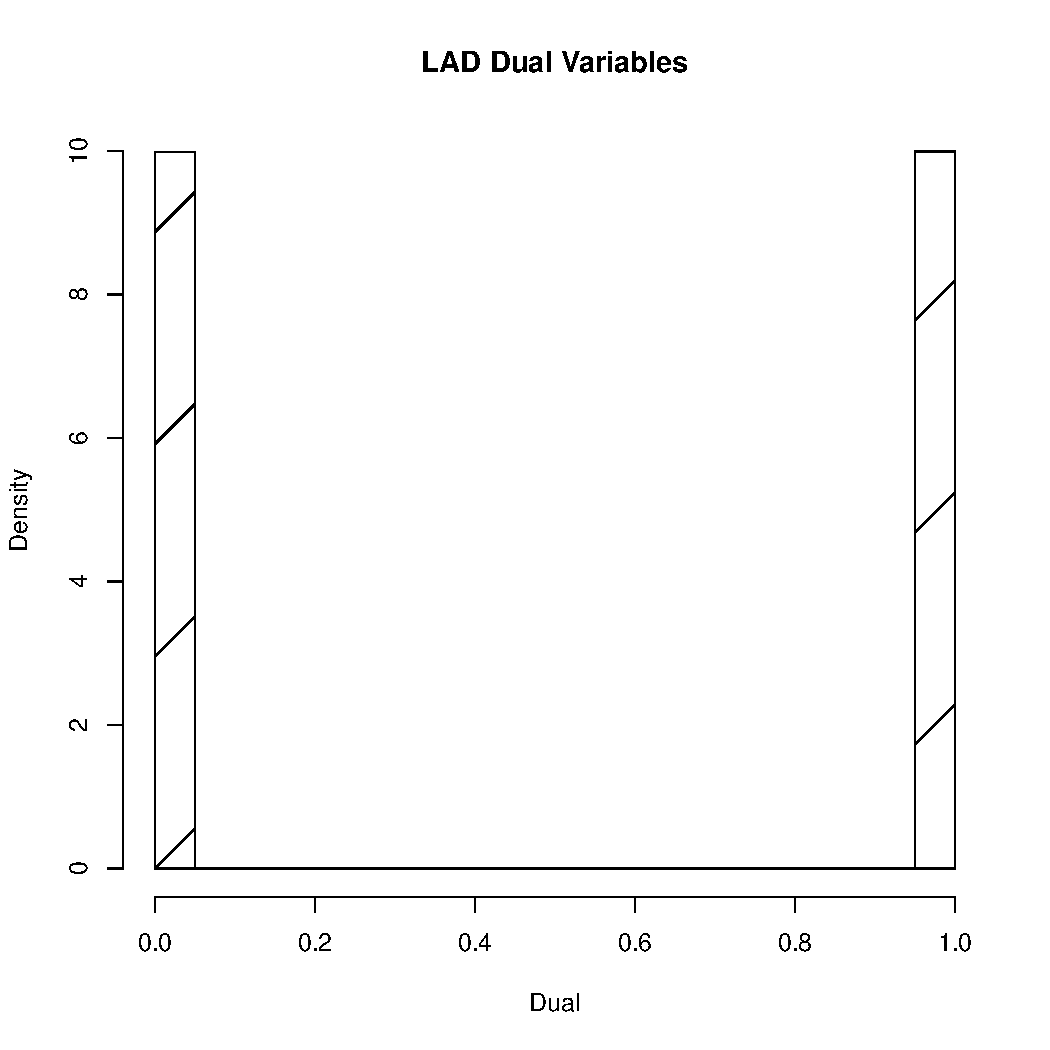
\includegraphics[width=8cm]{qNineHist.pdf}
\end{figure}

This makes sense, as we can think of the dual values as the cost to
the objective function for relaxing the constraint to which they
represent. The constraints for the quantile regression primal are that
$Y_i - X\beta + u_i - v_i = 0$. If this constraint is relaxed say by
increasing $Y_i$, the objective function benefits if $u_i > 0$, and
does not benefit if $v_i > 0$. We can see this because if $u_i > 0$,
then $Y_i - X\beta < 0$. Increasing $Y_i$ improves the fit, and allows for
a smaller value of $u_i$ to meet the constraint. This gives a benefit
of $\tau$. However if $v_i > 0$, then $Y_i - X\beta > 0$ and we must increase
$v_i$ in order to maintain the equality of the constraint. When this
occurs, the dual variable corresponding to the constraint will be $1$,
and when $u_i > 0$, we will see that the dual variable is $0$. The
constraints for which $u_i = v_i = 0$ will have dual variables between
$0$ and $1$.


\section*{Question 10}

Given your findings from question 8, can you think of a way to recover
$\beta_{\tau}$ for some $\tau$ using only $h$ observations from the data set,
where $h$ is defined as in question 8.

\vspace{.3in}

If we know the 16 points for which there is no residual value, and
there are 16 dimensions to $\beta$, then there is a perfectly identified
system for $\beta$. Define $X_h$ to be the matrix of covariates containing
only the 16 rows that are in $h$. Likewise define $Y_h$.

We know that $Y_h = X_h \beta$ as all of these points have zero
residuals. But $X_h$ is a $16 \times 16$ matrix by construction, and by
assumption contains no perfect colinearity so we may invert this
matrix. Then $\beta = \inv{X_h} Y$.


\end{document}
